\section{Spieltheorie II: Vertiefung und Anwendung}

In dieser Vorlesung wird die Spieltheorie der 2-Personen Spiele vertieft
werden. Da im Rahmen dieser Vorlesung nicht genug Raum für eine umfassende 
Darstellung der Grundlagen der Spieltheorie bleibt, wird die
Spieltheorie auch diesmal nicht systematisch entwickelt, sondern über Beispiele
eingeführt. Weiterhin werden am Beispiel des Gefangenendilemmas wiederholte
Spiele besprochen werden. Schließlich wird, wiederum anhand von Beispielen, auf
Anwendungsmöglichkeiten der Spieltheorie eingegangen werden.

\subsection{Nicht-Nullsummenspiele}

Bereits in der letzten Vorlesung haben wir mit dem Ver\-trauens\-spiel, dem
Hirsch\-jagd\-spiel und dem Gefangenendilemma Beispiele für
Nicht-Nullsummenspiele besprochen. Um die Erörterung der folgenden Beispiele
wenigstens etwas zu systematisieren, kann zunächst zwischen Koordinations- und
Nicht-Koordinationsspielen unterschieden werden. {\em Koordinationsspiele} sind
solche Spiele, bei denen die Spieler sich bloß koordinieren müssen, um ein für
sie wünschenswertes Ergebnis zu erreichen bzw. ein für alle Beteiligten nicht
wünschenswertes Ergebnis zu vermeiden. Gelingt es Ihnen aber, sich zu
koordinieren, dann werden sie -- schon aus Eigeninteresse -- bei der gewählten
Lösung bleiben. Ein Beispiel für ein Koordinationsspiel ist das
Hirschjagdspiele (siehe Seite \pageref{Hirschjagdspiel}).
"`Nicht-Koordinationsspiele"' wären dementsprechend alle anderen Spiele. Für
uns sind dabei besonders solche Spiele von Interesse, die ein echtes {\em
Kooperationsproblem} modellieren, wie z.B. das Gefangenendilemma. Echte
Kooperationsprobleme sind, grob gesagt, solche Probleme, bei denen die für alle
Beteiligten wünschenswerte Lösung kein Gleichgewicht ist, d.h. die Spieler
haben einen Anreiz aus Eigeninteresse von der wünschenswerten Lösung 
abzuweichen. So ist die wechselseitge Kooperation im Gefangenendilemma,
obwohl sie aus Sicht beider Spieler wünschenswert wäre, nicht stabil, da jeder
der Spieler sich verbessern kann, wenn er selbst nicht kooperiert, 
vorausgesetzt der andere bleibt bei
seiner Strategiewahl.

Es stellt sich die Frage, was in diesem Zusammenhang "`wünscheswert"' bzw.
"`wünschenswerte Lösung"' heißt. Daraus könnte man nun wieder eine der
philosophischen Frage machen, zu der die Meinungen weit auseinandergehen
können. Immerhin gibt es aber ein recht naheliegendes {\em notwendiges
Kriterium} für das, was eine "`wünschenswerte Lösung"' ist, nämlich das aus den
Wirtschaftswissenschaften bekannte Kriterium der {\em Pareto-Optimalität}. Im Zusammenhang der
Spieltheorie ist ein Ergebnis "`pareto-optimal"' wenn es kein andere Ergebnis gibt, bei dem
wenigstens einer der Spieler eine höhre Auszahlung bekommt und kein anderer
eine niedrigere. Dass die Pareto-Optimalität ein sinnvolles notwendiges
Kriterium für ein "`wünschenswertes Ergebnis"' darstellt, wird daraus deutlich,
dass ein nicht pareto-optimaler Zustand ein Zustand ist, in dem man
wenigstens einen Spieler besser stellen könnte, ohne dass ein anderer Spieler
schlechter gestellt werden müsste. Dann ist es aber sicher nicht
"`wünschenswert"' bei einem Zustand zu verbleiben, 
den man so leicht und ohne Nachteile in Kauf nehmen zu müsssen, verbessern
könnte.

Andererseits ist einzuräumen, dass man sich auch Beispiele vorstellen kann, in
denen eine Gleichverteilung von Gütern unbedingt wünschenswerter ist als eine
Ungleichverteilung, selbst wenn man sie gegen eine Art von Ungleichheit
eintauschen könnte bei der niemand gegenüber der Gleichheit schlechter gestellt
wird. In diesem Zusammenhang ist auch darauf hinzuweisen, dass das
Pareto-Kriterium in erster Linie ein (kollektives) Effizienzkriterium und kein
Gerechtigkeitskriterium ist. Wenn wir 100 Euro an zwei Personenn verteilen
sollen und geben einer Person 1 Euro und der anderen 99 Euro, dann ist die
Verteilung ebenso paretoeffizient wie diejenige, bei der beide Personen 50 Euro
bekommen, obwohl die letztere von den vielen Menschen als die gerechtere beurteilt werden
dürfte. Man kann noch einen Schritt weitergehen und fragen, ob es nicht besser
wäre -- wenn man nur eine der beiden folgenden Alternativen hat -- lieber beiden
40 Euro geben und 20 Euro zum Fenster hinaus zu werfen, als zuzulassen, dass
eine Person 99 Euro an sich reisst und die andere nur einen Euro
bekommt. (Dies ist in nuce eins der Argumente, mit dem man die
Rechtfertigugn von möglicherweise ineffizienten Umverteilungsbürokratien
versuchen könnte.) Schließlich könnte man die Frage aufwerfen, wie man eine
Situation handhaben sollte, in der 100
Euro nur in Form von 20 Euro-Scheinen verfügbar sind. Angenommen, beide Personen
haben schon jeweils 40 Euro bekommen. Was soll nun mit den restlichen 20 Euro geschen.
Soll man einer Person 60 Euro geben, um einen pareto-effizienten Zustand zu
schaffen und "`nichts verkommen zu lassen"'. Oder sollte man die restlichen 20
Euro feierlich verbrennen, um keine Ungerechtigkeiten entstehen zu
lassen?
% \footnote{Dazu gibt es noch folgende hübsche Geschichte, die das Verhältnis von Theorie und
% Praxis in den Wirtschaftswissenschaften beleuchtet, aber von der ich leider
% nicht mehr weiss, wo ich sie gelesen habe: "`Ein Vater geht mit seinen beiden Kindern 
% zum Kiosk, um Eis am Stil für die Kinder zu kaufen. Das Geld würde für drei Eis reichen, doch
% wohlweislich kauft der Vater jedem Kind nur ein Eis. Daraufhin wird er von dem
% Kioskbesitzer, der ein diplomierter Wirtschaftswissenschaftler ist, darüber
% belehrt, dass sein Verhalten einen parto-ineffizienten Zustand herbeigeführt
% habe, denn er könne ohne Weiteres einem der Kinder noch einer zusätzliches Eis
% kaufen, ohne dass das andere Kind deswegen schlechter gestellt wäre. Der Vater
% folgt diesem gut gemeinten Ratschlag des ökonomisch kompetenten
% Kioskbesitzers. Wie zu befürchten, hebt darauf jedoch ein großes Geplärr unter
% den Kindern an. Die Vorhaltungen des Vaters, der dem Ratschlag des Ökonomen
% die Schuld am Streit unter den Kindern gibt, kontert der Kioskbesitzer
% gelassen mit dem Hinweis, dass es offenbar versäumt habe, seine
% Kinder frühzeitig zu rationalem Verhalten zu erziehen."'}

Diese Überlegungen sollen nur zeigen, dass das Kriterium der Pareto-Effizienz
nicht zwingenderweise in allen Situationen ein taugliches Kriterium dafür ist,
was besser oder wünschenswerter ist. Dennoch hat das Kriterium der
Pareto-Effizienz im Allgemeinen eine hohe Plausibilität, weshalb wir auch im
Folgenden darauf zurückgreifen werden. Es ist jedoch wichtig, sich der Grenzen
bewusst zu bleiben.


\subsubsection{Koordinationsspiele}

Koordinationsspiele sind dadurch gekennzeichnent, dass es mehrere
Nash-Gleichgewichte (in reinen Strategien) gibt, von denen wenigstens eins
pareto-effizient ist. Dabei können zwei Arten von Koordinationsproblemen
entstehen: 1) Wenn es nur ein pareto-effizientes Gleichgewicht gibt, müssen
sich die Spieler so koordinieren, dass sie das pareto-effiziente Gleichgewicht
erreichen und nicht in einem anderen Gleichgewicht gefangen werden. 2) Wenn es
mehrere pareto-effiziente Gleichgewichte gibt, dann müssen sich die Spieler
irgendwie auf eins der Gleichgewichte einigen. Misslingt die Einigung, so kann
es dazu kommen, dass sie die Gleichgewichte überhaupt verfehlen.

\paragraph{Hirschjagdspiel als Koordinationsspiel} Ein Beispiel für das erste
Problem ist das in der letzten Woche schon vorgestellte Hirschjagdspiel:
\begin{center}
\begin{tabular}{cc|c|c| c|c|c|}
& \multicolumn{1}{c}{} & \multicolumn{2}{c}{\bf Jäger 2} 
& \multicolumn{1}{c}{} & \multicolumn{2}{c}{\bf Jäger 2} \\
& \multicolumn{1}{c}{} 
& \multicolumn{1}{c}{Hirsch} & \multicolumn{1}{c}{Hase} 
& \multicolumn{1}{c}{} 
& \multicolumn{1}{c}{Hirsch} & \multicolumn{1}{c}{Hase} 
\\ \cline{3-4} \cline{6-7}
& Hirsch   & {\bf 5, 5, 5} & 0, 2, 0 & &  0, 0, 2 & 0, 2, 2 \\
\cline{3-4} \cline{6-7}
\raisebox{1.5ex}[-1.5ex]{{\bf Jäger 1}} 
& Hase     & 2, 0, 0 & 2, 2, 0 & &  2, 0, 2 & {\bf 2, 2, 2} \\
\cline{3-4} \cline{6-7}
\multicolumn{7}{c}{} \\
& \multicolumn{1}{c}{} & \multicolumn{2}{c}{{\small {\bf Jäger 3}: Hirsch}}
& \multicolumn{1}{c}{} & \multicolumn{2}{c}{{\small {\bf Jäger 3}: Hase}} \\
\end{tabular}
\end{center}
In diesem Spiel gibt es zwei Nash-Gleichgewichte: 
\begin{enumerate}
  \item Gleichgewicht ("`Hirschjagdgleichgewicht"'): Alle Jäger jagen den
  Hirsch.
  \item Gleichgewicht ("`Hasenjagdgleichgewicht"'): Alle Jäger jagen Hasen.
\end{enumerate}
Dass es sich um Nash-Gleichgewichte handelt,
geht aus folgender Überlegung hervor: 
\begin{enumerate} 
  \item Gleichgewicht: Wenn alle Jäger den
Hirsch jagen, hätte kein Jäger einen Grund als einziger einen Hasen zu jagen, weil dann sein
Braten wesentlich kleiner ausfällt (Nutzenwert von zwei statt von fünf).
 
\item Gleichgewicht: Wenn alle Jäger Hasen jagen, hat keiner der Jäger einen Grund im
Alleingang auf die Hirschjagd zu gehen, weil er alleine den Hirsch ohnehin nicht fangen kann.

\item Alle anderen Ergebnisse: In allen anderen Fällen versuchen nur einige
Jäger den Hirsch zu jagen. Da kein Jäger den Hirsch ohne die Mithilfe aller
fangen kann, kann ein Jäger, der vorhatte, den Hirsch zu jagen, sein Ergebnis
verbessern, indem er auf die Strategie des Hasenjagens umstellt. Wenn
wenigstens ein Spieler einen Anreiz hat, seine Strategie im Alleingang zu
ändern, handelt es sich nicht mehr um einen Gleichgewichtszustand. Also gibt es
außer den beiden genannten Gleichgewichten kein weiteres Nash-Gleichgewicht
mehr.
\end{enumerate}

Das einzige paretoeffiziente Ergebnis dieses Spiels bildet das
Hirschjagdgleichgewicht. Auch davon kann man sich leicht überzeugen. Denn egal
welches andere Ergebnis man aus der Tabelle heranzieht, beim
Hirschjagdgleichgewicht sind alle Jäger im Vergleich dazu besser gestellt
(sie erhalten einen Nutzenwert von fünf anstelle von zwei oder null).
Insbesondere ist auch das Hasenjagdgleichgewicht kein paretoeffizientes
Ergebnis, auch wenn es eine Pareto-Verbesserung gegenüber allen anderen
Ergebnissen bis auf das Hirschjagdgleichgewicht darstellt.

Das Koordinationsproblem beim Hirschjagdspiel besteht
darin, dass das paretoeffiziente Hirschjagdgleichgewicht sehr viel instabiler ist als das
Hasenjagdgleichgewicht. Wenn wir unter dem {\em Anziehungsbereich} eines
Gleichgewichtes die Menge aller derjenigen Strategiekombinationen verstehen, die
man durch eine endliche Anzahl von nutzenerhöhenden Strategiewechseln
jeweils einzelner Jäger in das Gleichgewicht überführen kann, dann sieht man
leicht, dass der Anziehungsbereich des Hasenjagdgleichgewichts wesentlich
größer ist als der des Hirschjagdgleichgewichts. Zum Anziehungsbereich des
Hasenjagdgleichgewichts gehören alle Strategiekombinationen bis auf das
Hirschjagdgleichgewicht. Diejenigen Strategiekombinationen, bei denen
mehr als ein Jäger auf Hasenjagd geht, gehören sogar ausschließlich zum
Anziehungsbereich des Hasenjagdgleichgewichts. Dagegen gehören zum
Anziehungsbereich des Hirschjagdgleichgewichts nur diejenigen Strategiekombinationen, bei denen
höchstens ein Jäger auf Hasenjagd geht. Und selbst diese Strategiekombinationen
gehören nicht ausschließlich zum Anziehungsbereich des
Hirschjagdgleichgewichts, sondern ebenso auch zum Anziehungsbereich des
Hasenjagdgleichgewichts. (Woran man gleichzeitig sieht, dass sich die
Anziehungsbereiche der Gleichgewichte am Rand überschneiden können.)

Es ist charakteristisch für Koordinationsprobleme im Gegensatz zu den unten zu
besprechenden Kooperationsproblemen, dass sie sich theoretisch allein durch
Verabredungen, Signale oder Konventionen lösen lassen, ganz ohne jeden
Bestrafungs- bzw. Sanktionsmechanismus. Das beliebte Schlagwort "`Talk ist
Cheap"' (soll heißen: Ein Versprechen zu geben kostet nichts, weil man es später
sowieso brechen kann) gilt nur bei Kooperationsproblemen aber nicht bei
Koordinationsproblemen.

\paragraph{Widerstreitende Ziele ("`Clash of Wills"')} Ein vergleichsweise
schwächeres Koordinationsproblem stellt das Spiel der "`Widerstreitenden
Ziele"' dar (welches in der älteren Literatur auch oft unter dem Titel "`Kampf
der Geschlechter"' auftaucht). Hier ist die Geschichte zum Spiel: Fred und
Clara wollen am Abend zusammen ausgehen. Sie telefonieren 
deswegen miteinander und überlegen, wo sie hingehen könnten. Freq möchte am
liebsten die Oper besuchen. Clara dagegen findet die Oper ein wenig langweilig
und würde es vorziehen, zu den Chippendales zu gehen. Allerdings würde sie
immer noch lieber zusammen mit Fred in die Oper gehen anstatt alleine zu den
Chippendales. Und umgekehrt würde auch Fred sich notfalls zu den Chippendales
schleppen lassen, wenn er dadurch immerhin den Abend an Claras Seite verbringen
darf. Bevor sie zu einer Einigung kommen ist leider der Akku von Freds Handy
leer. Jeder von beiden überlegt für sich, wo er bzw. sie am Abend hingehen
sollten, um den anderen zu treffen. Daraus ergibt sich die Spielmatrix:

\begin{center}
\begin{tabular}{cc|c|c|}
& \multicolumn{1}{c}{} & \multicolumn{2}{c}{\bf Clara} \\
& \multicolumn{1}{c}{} & \multicolumn{1}{c}{Oper} &
                             \multicolumn{1}{c}{Chippendales} \\ \cline{3-4} 
& Oper                 & {\bf 2, 1}                & 0,0  \\ \cline{3-4}
\raisebox{1.5ex}[-1.5ex]{{\bf Fred}} 
& Chippendales         & -1,-1                     & {\bf 1,2} \\ \cline{3-4}
\end{tabular}
\end{center}

Wie man leicht nachprüfen kann, gibt es in diesem Spiel zwei reine
Nash\-gleich\-ge\-wichte in den Strategiekombonationen $(Oper, Oper)$ und
$(Chippendales, Chippendales)$. Beide Nashgleichgewichte sind zudem
paretoeffizient, während alle anderen reinen Strategiekombinationen
paretoineffizient sind. Weiterhin existiert ein gemischtes Gleichgewicht, denn
sei $p$ die Wahrscheinlichkeit, mit der Fred am Abend in der Oper erscheint,
dann bestimmt sich Claras Erwartungsnutzen für jede ihrer reinen Strategien
nach:
\begin{eqnarray*}
EW(Clara)_{Oper} & = & p \cdot 1 + (1-p) \cdot (-1) \\
EW(Clara)_{Chippendales} & = & p \cdot 0 + (1-p) \cdot 2 
\end{eqnarray*}
Wenn Claras Gleichgewichtsstrategie ebenfalls eine gemischte Strategie sein
soll, dann muss sie zwischen ihren reinen Strategien indifferent sein, da sie
andernfalls die bessere der reinen Strategien wählen würde. Dann kann man beide
Werte  gleichsetzen und erhält:
\begin{eqnarray*}
EW(Clara)_{Oper} & = & EW(Clara)_{Chippendales} \\
p \cdot 1 + (1-p) \cdot (-1) & = & p \cdot 0 + (1-p) \cdot 2 \\
2p - 1 & = & 2 - 2p \\
p & = & \frac{3}{4}
\end{eqnarray*}
Freds gemischte Gleichgewichtsstrategie besteht also darin, mit einer
Wahrscheinlichkeit von $p=3/4$ zur Oper zu gehen. Da das Spiel vollkommen
symmetrisch ist, besteht Claras gemischte Gleichgewichtsstrategie darin, mit
einer Wahrscheinlichkeit von $q=3/4$ die Chippendales zu besuchen. Der
Nutzenwert für Fred und Clara im gemischten Gleichgewicht ist für beide $1/2$.
Das gemischte Gleichgewicht ist also nicht paretoeffizient, weil beide davon
profitieren würden, zu einem der reinen Gleichgewichte überzugehen. Trotzdem
handelt es sich um ein Gleichgewicht, da keiner von beiden einen positiven
Anreiz hat, im Alleingang von der gemischten Strategie zu einer der reinen
Strategien überzugehen oder eine andere gemischte Strategie, d.h. eine mit
einem anderen Wahrscheinlichkeitswert, zu wählen.

Bedeutet das nun so etwas wie, dass es für Clara und Fred auf jeden Fall besser
ist, eine ihrer reinen Strategien zu wählen, als den Zufall entscheiden zu
lassen? Das Koordinationsproblem wird damit nicht aus der Welt geschafft, denn
keiner von beiden weiss ja, für welche reine Strategie der andere sich
entscheiden wird. Wenn Clara und Fred irgendwann einmal gelernt haben, dass man
bei Unwissen gemäß dem Indifferenzprinzip davon ausgehen soll, dass alle
Möglichkeiten gleichverteilt sind, dann würde das nur dazu führen, dass sie
genau das Falsche tun, denn wenn man die Wahrscheinlichkeit, mit der der andere
jede seiner Strategien wählen wird, mit 50\% veranschlagt, dann wäre es für
Clara das Beste zu den Chippendales zu gehen und für Fred, die Oper aufzusuchen.
Wie man sich leicht überlegen kann, ist mit dem Wissen über das -- ohnehin
nicht einmal paretoeffiziente -- gemischte Gleichgewicht in dieser Situation
ebenfalls nichts anzufangen. Setzt Clara z.B. voraus, dass Fred entsprechend
seiner gemischten Gleichgewichtsstrategie randomisiert, dann ist es für sie
vollkommen gleich wohin sie geht, was das Koordinationsproblem auch nicht löst. 

Es würde nichts dagegen sprechen, wenn Clara und Fred eine Münze werfen, um zu
entscheiden, wohin sie gehen. Nur hilft es leider nicht, wenn jeder für sich
eine Münze wirft. Sie müssten es schon beide gemeinsam tun. Da sie sich der
Situationsbeschreibung nach aber aufe keine {\em koordinierte Strategie} mehr
verständigen können, fällt diese Lösung aus. 

Das Problem wäre womöglich weniger gravierend, wenn das Spiel nicht vollkommen
symmetrisch wäre. Wenn z.B. der Nutzenwert von Fred für einen Opernbesuch
deutlich höher wäre als der Nutzen, den Clara aus den Chippendales bezieht, und
wenn dies beiden bekannt ist, und wenn beiden bekannt ist, dass es beiden
bekannt ist, dann wäre es sicherlich für jeden von beiden naheliegend, vor der
Oper zu erscheinen. Ist die Situation aber vollkommen symmetrisch, dann stellt
sich das Koordinations-Problem als ein Problem des {\em Symmetriebruchs}
dar.\footnote{Die klassische Geschichte zum Problem des Symmetriebruchs ist
die von "`Buridans Esel"': Der Esel steht genau in der Mitte zwischen zwei
gleich großen Heuhaufen, da er sich nicht entscheiden kann, welchen er fressen
soll, verhungert der Esel.} Als Mechanismen zum Symmetriebruch wirken häufig
gesellschaftliche oder individuelle Konventionen. Zum Beispiel könnten beide
sich nach dem Prinzip "`Lady's first"' jeweils dafür entscheiden, die
Chippendales zu besuchen. Oder bisher hat sich Clara immer als die dominantere
erwiesen, so das Fred und Clara beide davon ausgehen, dass sie sich -- hätte das
Telefongespräch länger gedauert -- sowieso für die Chippendales entschieden.

\subsubsection{Nicht Koordinations-Spiele}

Die Spiele, die keine Koordinationsspiele sind, bilden natürlich eine ziemlich
große und disparate Gruppe. Im folgenden werden beispielhaft zwei Spiele
besprochen, die vergleichsweise schärfere Dilemmata abbilden, als das bei
Koordinationsspielen der Fall ist.

\paragraph{Das Angsthasen-Spiel ("`Chicken-Game"')} 

Wie üblich als erstes die Geschichte zum Spiel: Beim Angsthasen-Spiel müssen
die beiden "`Spieler"' mit Ihren Autos mit hoher Geschwindigkeit frontal
aufeinander zufahren. Wer zuerst ausweicht ist ein "`Angsthase"' und hat verloren.
Wenn keiner ausweicht, kommt es zum Unfall. Daraus ergibt sich die Spielmatrix:

\begin{center}
\begin{tabular}{c|c|c|}
\multicolumn{1}{c}{} & \multicolumn{1}{c}{Ausweichen} &
                               \multicolumn{1}{c}{Gas geben } \\ \cline{2-3} 
Ausweichen               & 0, 0           & {\bf -5,5}      
\\ \cline{2-3} 
Gas geben                & {\bf 5,-5}     & -100,-100
\\ \cline{2-3}
\end{tabular}
\end{center}

Das Spiel hat zwei reine Gleichgewichte nämlich $(Ausweichen, Gas geben)$ und
$(Gas geben, Ausweichen)$ mit den Auszahlungen $(-5,5)$ und $(5,-5)$. Ein
gemischtes Gleichgewicht existiert ebenfalls (siehe Übungsaufgabe
\ref{chickenGameAufgabe}).

Es ist offensichtlich, dass es für jeden Spieler im Zweifelsfall immer noch
besser ist auszuweichen als Gas zu geben. Zugleich ist es aber auch besser Gas
zu geben, wenn man Anlass zu der Annahme hat, dass der andere ausweicht. Daraus
entstehen zwei Probleme. Das erste Problem für beide Spieler besteht darin
überhaupt die Strategiekombination zu vermeiden, die zu dem Ergebnis
$(-100,-100)$ führt. Das zweite Problem besteht für jeden Spieler darin, das
für ihn vorteilhaftere der beiden Gleichgewichte herbei zu führen. Anders als
bei einem Koordinationsspiel lassen sich diese Problem nicht einfach durch eine
Absprache lösen. Denn auch wenn jeder der Spieler verspricht auszuweichen, so
ist doch zu befürchten, dass es sein Versprechen bricht im Vertrauen darauf,
dass der anderes seins halten wird. Bei einem Koordinationsspiel würde sich
jeder Spieler schon aus Eigeninteresse an das gegebene Versprechen halten. Ein
ähnliches Problem stellt sich aber auch, wenn ein Spieler, um den anderen zum
Nachgeben zu bewegen (und damit das für ihn selbst günstigere
Gleichgewicht herbei zu führen) schwört, dass er niemals nachgeben wird. Diese
Drohung ist nicht glaubwürdig, sofern sie nicht mit irgendeiner Art von
Selbstbindungsmechanismus verbeunden ist, die ihre Durchführung erzwingt, denn
es entspricht ansonsten garnicht der Interessenlage des Spielers, die eigene
Drohung wahrzumachen, sollte der Andere sie ignorieren.


\paragraph{Noch einmal Gefangenendilemma} Als ein weiteres Beispiel für ein
echtes Kooperationsproblem im Gegensatz zu einem bloßen Koordinationsproblem haben
wir bereits in der letzen Woche das Gefangenendilemma kennen gelernt:
\begin{center}
\begin{tabular}{c|c|c|}
\multicolumn{1}{c}{} & \multicolumn{1}{c}{Kooperieren} &
                                \multicolumn{1}{c}{Defektieren} \\ \cline{2-3} 
Kooperieren          & 3, 3                   & 0, 5  \\ \cline{2-3}
Defektieren          & 5, 0                   & 1, 1 \\ \cline{2-3}
\end{tabular}
\end{center}
In allgemeinerer Form kann das (symmetrische) durch die vier Parameter
$T$ ("`Temptation"), $R$ ("`Reward"'), $P$ ("`Punishment"') und $S$ ("`Sucker's
Payoff"') definiert werden:
\begin{center}
\setlength{\parskip}{0.25cm}
\begin{tabular}{c|c|c|}
\multicolumn{1}{c}{} & \multicolumn{1}{c}{Kooperieren} &
                                \multicolumn{1}{c}{Defektieren} \\ \cline{2-3} 
Kooperieren          & R, R                   & S, T  \\ \cline{2-3}
Defektieren          & T, S                   & P, P \\ \cline{2-3}
\end{tabular}
\label{GefangenendilemmaTabelle}

Gefangenendilemma-Bedingung: $T > R > P > S$
\end{center}

Im Gefangenendilemma existiert genau ein Nash-Gleichgeweicht, nämlich die
wechselseitige Defektion. Das Nash-Gleichgewicht ist aber nicht pareto-optimal,
da beide Spieler besser gestellt wären, würden sie miteinander kooperieren. Das
Gefangenendilemma beschreibt also eine Situation, in der individuelles
nutzenmaximierendes Verhalten zu einem Zustand führt, bei dem alle am
Ende schlechter gestellt sind. Gefangenendilemmasituationen treten
typischerweise auf, wenn irgendwelche Ressourcen gemeinsam genutzt werden. Eine
solche Resource ist, auch wenn der Ausdruck "`Resource"' darauf nicht so recht
passen mag, die öffentliche Ordnung und Sicherheit. Jedem leuchtet es ein, dass
es am besten ist, wenn alle Menschen ehrlich sind, und niemand dem anderen
etwas stiehlt. Aber am besten lebt es sich, wenn alle anderen Menschen ehrlich
sind, nur man selbst sich erlauben kann, die anderen zu bestehlen. Aber wenn
jeder so denkt, dann gibt es keine ehrlichen Menschen mehr. Das Problem der
öffentlichen Sicherheit wird bekanntermaßen durch Sanktionsmechanismen in Form
der Strafverfolgung gelöst. Ohne irgendeine Art von Sanktionsmechanismus lässt
sich das einfache Gefangenendilemma nicht lösen. Wir werden aber gleich sehen,
dass es sich "`lösen"' lässt,\footnote{Strenggenommen kann man hier nicht von
einer Lösung sprechen, da man lediglich von der Diskussion eines Spiels (des
einfachen Gefangenendilemmas) zu der eines anderen (des wiederholten
Gefangenendilemmas) übergegangen ist. Allerdings könnten sich in der
Wirklichkeit auftretende Gefangenendilemma-Situationen womöglich in der Tat
dadurch lösen lassen, dass man die "`Spielsituation"' in geeigneterweise
abändert.} wenn man von einfachen zu wiederholten Spielen übergeht.

\subsection{Wiederholte Spiele}

\subsubsection{Wiederholte Spiele am Beispiel des wiederholten
Gefangenendilemmas}

Im einfachen Gefangenendilemma ist, wenn man davon ausgeht, dass jeder Spieler
sich egoistisch-rational verhält, keine kooperative Lösung möglich. Aber wie
verhält es sich, wenn man das Spiel mehrfach wiederholt? Dann können die
Spieler darauf reagieren, wie sich ihr Gegenüber in der letzten Runde verhalten
hat. So kann ein Spieler die Kooperation in der folgenden Runde davon abhängig
machen, ob der andere in der gegenwärtigen Runde kooperiert oder nicht.
Inwiefern ändert das die strategische Situation? Angenommen, es wird ein
wiederholtes Gefangenendilemma von fünf Runden gespielt, und einer der Spieler
spielt die Strategie "`Wie Du mir, so ich Dir"' (englisch: "`Tit for Tat"'),
d.h. er kooperiert in der ersten Runde und kooperiert in den folgenden Runden
immer dann, wenn der Gegenüber in der vorhergehenden Runde ebenfalls kooperiert
hat. Welches Verhalten ist die beste Antwort auf "`Wie Du mir, so ich Dir"',
d.h. wie kann man gegen "`Wie Du mir, so ich Dir"' die höchste Auszahlung
erhalten? Spielt man -- analog zum einfachen Gefangenendilemma -- immer
unkooperativ, dann erhält man mit den Auszahlungsparametern der oben angegebenen
Spielmatrix die Auszahlungen:
\begin{center}
\begin{tabular}{|l|c|c|c|c|c|r|}
\cline{1-7}
Runde:       & 1 & 2 & 3 & 4 & 5 & $\sum$ \\
\cline{1-7}
Auszahlung:  & 5 & 1 & 1 & 1 & 1 & 9 \\
\cline{1-7}
\end{tabular}
\end{center}
Hätte man dagegen immer kooperativ gespielt, dann wären die Auszahlungen höher
ausgefallen:
\begin{center}
\begin{tabular}{|l|c|c|c|c|c|r|}
\cline{1-7}
Runde:       & 1 & 2 & 3 & 4 & 5 & $\sum$ \\
\cline{1-7}
Auszahlung:  & 3 & 3 & 3 & 3 & 3 & 15 \\
\cline{1-7}
\end{tabular}
\end{center}
Daraus wird deutlich, dass im wiederholten Gefangenendilemma unbedingte
Defektion keine dominante Strategie ist. Ist aber umgekehrt eine Strategie, die
gegen "`Wie Du mir so ich Dir"' immer kooperiert eine beste Antwort auf "`Wie
Du mir, so ich Dir"'. Sie ist es zumindest dann nicht, wenn man durch
irgendeine Änderung der Zugfolge ein besseres Ergebnis gegen "`Wie Du mir, so
ich Dir"' erziehlen kann. Das ist aber in der Tat möglich, wenn man nur in der
letzten Runde defektiert und bis dahin kooperiert. Dann ergibt sich:
\begin{center}
\begin{tabular}{|l|c|c|c|c|c|r|}
\cline{1-7}
Runde:       & 1 & 2 & 3 & 4 & 5 & $\sum$ \\
\cline{1-7}
Auszahlung:  & 3 & 3 & 3 & 3 & 5 & 17 \\
\cline{1-7}
\end{tabular}
\end{center}
Es lohnt sich also immer, in der letzten Runde zu defektieren. Und dies gilt
sogar nicht nur gegen die Strategie "`Wie Du mir, so ich Dir"', sondern gegen
schlechthin jede Strategie, denn auch gegen eine Strategie, die ihrerseits in
der letzten Runde defektiert, ist es besser in der letzten Runde zu defektieren
(und eine Auszahlung von 1 zu bekommen) als zu kooperieren (und eine Auszahlung
von 0) zu erhalten. Das ist auch keineswegs verwunderlich, denn für sich
betrachtet, stellt die letzte Runde ein einfaches Gefangenendilemma dar, und im
einfachen Gefangenendilemma ist Defektion, wie wir gesehen haben, die dominante
Strategie. Daraus ergibt sich aber eine wichtige Schlussfolgerung: Wenn in der
letzten Runde Defektion die dominante Strategie ist, dann müssten beide
Spieler, sofern sie sich strikt nutzenmaximierend verhalten, in der letzten
Runde stets defektieren. Wenn sie aber in der letzten Runde stets defektieren,
dann hat der Zug, den man in der vorletzten Runde spielt, keinen Einfluss mehr
darauf, wie der Gegner in der letzten Runde antwortet (sofern der Gegner sich,
wie gesagt, strikt nutzenmaximierend verhält). Mit anderen Worten man braucht
in der vorletzten Runde keine Belohnung für Kooperation durch den Gegner in der 
folgenden Runde mehr zu erhoffen, man muss aber auch die Bestrafung
für Defektion nicht mehr fürchten, da sie ohnehin eintritt. Dann befinden wir
uns aber auch in der vorletzten Runde in genau derselben Situation wie in der
letzten Runde, indem wir auf die zukünftige Reaktion des Gegners keine
Rücksicht nehmen müssen. Dann ist es aber das beste, auch in der vorletzten
Runde schon zu defektieren. Nun wiederholt sich dieselbe Überlegung auch für
die vorvorletzte Runde. Auch in der vorvorletzten Runde sollte man also --
wechselseitige strikte Rationalität vorausgesetzt! -- defektieren usw., so dass
schließlich jeder Spieler schon ab der ersten Runde defektieren müsste. Diese
Art von Argumention bei wiederholten Spielen, bei der man von der letzten Runde
rückwärts auf die vorletzte schließt, und von der vorletzten auf die
vorvorletzte bis man schließlich bei der ersten Runde angekommen ist,
bezeichnet man auch als {\em Rückwärtsinduktion}.

Die Rückwärtsinduktion zeigt uns also, dass strikt-rationale Spieler
auch im wiederholten Gefangenendilemma schon ab der ersten Runde defektieren
werden, sofern der Gegenüber sich ebenfalls strikt rational verhält und sofern
beiden bekannt ist, dass sie sich beide strikt rational verhalten. Diese
Bedingungen sind keine unwesentlichen Einschränkungen: Anders als im einfachen
Gefangenendilemma ist ausschließliche Defektion keine dominante Strategie --
dann wäre sie die beste Strategie, egal ob der Gegner sich rational verhält
oder nicht, und unabhäbgig davon, was über das Verhalten des Gegners bekannt
ist -- sondern lediglich eine Gleichgewichtsstrategie. Gibt es auch nur
geringen Anlass daran zu zweifeln, dass der Gegenspieler sich strikt
rational verhält (z.B. indem er auch in der letzten Runde Kooperation noch
kooperiert, wenn kein besonderer Grund dagegen spricht), dann greift das
auf die Rückwärtsinduktion gestützte Argument schon nicht mehr.

Zudem setzt das Argument voraus, dass die Rundenzahl bekannt ist. Ist die
Rundenzahl unbekannt (z.B. wenn das Spiel nicht durch die Anzahl der
Wiederholungen, sondern durch eine Abbruchwahrscheinlichkeit nach jeder Runde
begrenzt wird), so lässt sich die Argumentation ebenfalls nicht anwenden. Damit
gilt aber insgesamt, dass es im wiederholten Gefangenendilemma nur im
Ausnahmefall rational ist, von der ersten Runde an ausschließlich zu
defektieren, nämlich dann, wenn entweder die Rundenzahl endlich und bekannt ist
{\em und} der Gegenspieler sich strikt rational verhält {\em und} überdies auch
seinerseits von der strikten Rationalität seines Gegenübers ausgeht, oder wenn die
Gegnerstrategie zufällig eine solche ist, gegen die ausnahmslose Defektion die
beste Antwort darstellt.

\subsubsection{Das "`Volkstheorem"' ("`folk theorem"')}

Wenn ausnahmslose Defektion im wiederholten Gefangenendilemma in aller Regel
nicht die beste Strategie ist, welches ist aber dann die beste Strategie? Die
Antwort lautet: Es gibt keine beste Strategie. Wie gut eine Strategie
abschneidet, hängt immer davon ab, auf welchen Gegner sie trifft. Dass es keine
beste Strategie gibt, lässt sich sehr leicht beweisen, indem man zeigt, dass
es zwei Strategien gibt, zu denen die besten Antwort-Strategien jeweils
verschieden sind. Diese beiden Strategien sind die Strategien "`Falke"' und
"`Unerbittlich"'. Die Strategie "`Falke"' defektiert ausnahmslos in allen
Runden. (Das Gegenstück dazu ist übrigens die Strategie "`Taube"', die
ausnahmslos kooperiert.) Die Strategie "`Unerbittlich"' kooperiert solange, bis der Gegner
ein einziges mal defektiert. Wenn das geschieht, dann defektiert sie ab der
folgenden Runde ausnahmslos für den gesamten Rest des Spiels. 

Nun kann man sich überlegen, dass die beste Antwort auf die Strategie "`Falke"'
nur eine Strategie sein kann, die gegen "`Falke"' ab der ersten Runde ausnahmslos
defektiert. Das bedeutet nicht, dass sie auch gegen andere Strategien
ausnahmslos defektieren muss. (Sie könnte, z.B. wenn die Gegnerstrategie ein
Kooperationsangebot macht, ihrerseits auf Kooperation umschwenken.) Aber
zumindest in der ersten Runde muss sie unbedingt defektieren, sonst würde sie
in der ersten Runde gegen "`Falke"' Punkte verschwenden, womit sie keine beste
Antwort auf "`Falke"' mehr wäre.

Gegen "`Unerbittlich"' kann diese Strategie dann aber keine beste Antwort mehr
sein. Den jede beste Antwort auf "`Unerbittlich"' muss gegen "`Unerbittlich"' ab
der ersten Runde kooperieren. Damit ist gezeigt, dass es im wiederholten
Gefangenendilemma keine stark oder schwach dominante Strategie gibt.

Wie sieht es aber mit Gleichgewichtsstrategien aus? Davon gibt es einem
bekannten Theorem der Spieltheorie zufolge unüberschaubar viele. Das Theorem,
um das es sich handelt, ist das sogennante Volkstheorem (englisch: "`folk
theorem"'; "`folk"', weil kein Erfinder des Theorems bekannt und es damit
gewissermaßen Allgemeingut ist). Das Folk-Theorem sagt nun nicht unmittelbar 
etwas darüber aus, welche Strategien in
wiederholten Spielen Gleichgewichtsstrategien sind, und welche nicht, aber es
sagt etwas über die möglichen Durchschnittsauszahlungen von Gleichgewichten in
wiederholten Spielen aus. In (vereinfachter Form) lautet das Folk-Theorem so:
\begin{quote}
{\em Volkstheorem}: In (unendlich oft) wiederholten Spielen ist jedes Resultat
erzielbar, das den Spielern mindestens ihren {\em Maximin-Wert} bietet.

{\footnotesize Dass ein Resultat "`erzielbar"' ist heisst dabei, dass es ein
Gleichgewicht gibt, bei dem das entsprechende Resultat heraus kommt. Unter dem "`Resultat"' sind dabei die
Durchschnittsauszahlungen zu verstehen, die die Spieler über das gesamte
wiederholte Spiel erhalten. Der Maximin-Wert ist derjenige Wert, den ein
Spieler erhält, wenn er "`auf Nummer sicher"' geht und so spielt, das er seinen
Verlust minimiert. (Vgl. dazu die Maximin-Regel bei Entscheidungen unter
Unwissenheit, S. \pageref{maximinRegel}.) Im (wiederholten) Gefangenendilemma
kann ein Spieler dadurch, dass er defektiert, sicherstellen, dass er mindestens
die Auszahlung für wechselseitige Defektion erhält. (Mit unseren Zahlen also
einen Nutzenwert von 1.)}
\end{quote}
Der {\em Beweis} der Volkstheorems lässt sich für den Sonderfall des
wiederholten 2-Personen Gefangenendilemmas etwa so führen: Wenn jedem Spieler
der Maximin-Wert garantiert werden soll, dann kann das Gleichgewichts-Resultat
für jeden der Spieler nur Werte von $P$ bis $R$ haben. Andernfalls (bei Werten
kleiner $P$ oder bei Werten größer $R$) müsste einer der Spieler freiwillig
auf den Minimax-Wert verzichten, obwohl er diesen Wert notfalls immer durch
Defektion erzwingen könnte. Sei $X$ nun irgendein Wert für den gilt: $P \leq X
\leq S$. Dann gibt es eine Zugfolge, die jedem Spieler die Auszahlung $X$ liefert.
(Beispiel: Angenommen $P=1$ und $S=3$ und $X=2\frac{1}{3}$, dann liefert die
Zugfolge $Kooperation, Kooperation, Defektion$ wenn sie von beiden Spielern
gespielt wird, jedem Spieler genau die Auszahlung $X=2\frac{1}{3}$.) Dann lässt
sich diese Zugfolge aber durch eine spezielle Variante der Strategie
"`Unerbittlich"' erzwingen, die selbst diese Zugfolge spielt und genau dann 
für den Rest des Spiels auf Bestrafung umschaltet, wenn der Gegenüber von
dieser Zugfolge ein einziges Mal abweicht. Wenn wir diese Variante
"`Unerbittlich*"' nennen, dann bildet das Strategiepaar (Unerbittlich*,
Unerbittlich*) ein Gleichgewicht, denn keiner der beiden Spieler kann von
seiner Gleichgewichtsstrategie abweichen, ohne mit einer schlechteren 
Durchschnittsauszahlung rechnen zu müssen.

\subsection{Evolutionäre Spieltheorie}

\subsubsection{Evolutionäre Spieltheorie am Beispiel des wiederholten
Gefangenendilemmas}

Das Modell des wiederholten Gefangenendilemmas war für lange Zeit eines der
populärsten Modelle der evolutionären Spieltheorie. Besonders duch den auf
Computersimulationen gestützten Ansatz von Robert Axelrod \cite[]{axelrod:1984}
ist es weithin bekannt geworden. Leider hat die Popularität dieses Modells zu
einer maßlosen Überschätzung seiner Leistungsfähigkeit geführt. Einer
unüberschaubaren Fülle von reinen Modell- und Simulationsstudien steht ein mehr
als auffälliger Mangel an empirischen Anwendungen gegenüber. Da das Modell aber
ebenso anschaulich wie leicht verständlich ist, werden wir es hier dennoch zur
Einführung in einige der Grundgedanken der evolutionären Spieltheorie
heranziehen. Auf die Probleme werden wir danach kurz eingehen.

Wie wir gesehen haben, existiert im wiederholten Gefangenendilemma keine
dominante Strategie und es gibt eine Vielzahl von Gleichgewichtsstrategien.
Können wir trotzdem irgendwelche Strategien als gute oder in irgendeinem anderen
Sinne als dem der Dominanz als "`beste"' Strategien auszeichnen. Der (aus
heutiger Sicht naive) Ansatz, den Axelrod verfolgt hat \cite[]{axelrod:1984},
bestand darin, einfach eine größere Menge von unterschiedlichen Strategien in
einer Art Turnier gegeneinander antreten zu lassen. Jede Strategie spielt gegen
jede andere ein paarweise Gefangenendilemma durch. "`Gewonnen"' hat am Ende die
Strategie, die die höchste Durchschnittspunktzahl über alle Begegnungen erzielt
hat. (Wohlbemerkt: Es kommt bei diesem Turnier auf die Durchschnittspunktzahl und
nicht auf die Anzahl gewonnenen Begegnunen bzw. der besiegten Gegner an, ganz wie
es dem ökonomischen Menschbild des "`neidlosen Egoisten"' entspricht.) Da man die
Strategien im wiederholten Gefangenendilemma sehr leicht programmieren kann,
führt man entsprechende Turniere am besten mit dem Computer durch.\footnote{Wen
es interessiert, der kann sich die Software dafür von dieser Web-Seite
herunterladen: http://www.eckhartarnold.de/apppages/coopsim.html }

Um das Prinzip zu verdeutlichen, wird an dieser Stelle nur ein sehr einfaches
Turnier mit einer sehr kleinen Stratgiemenge von 7 Strategien besprochen.
Diese ausgewählten Strategien sind:
\begin{itemize}
  \label{Strategien}
  \item {\em Grim} ("`Unerbittlich"'): Kooperiere in der ersten Runde;
  setze in den folgenden Runden die Kooperation fort, solange der Gegner
  kooperiert; Defektiere bis zum Ende der Begegnung, wenn der Gegner ein
  einziges Mal defektiert hat.
  \item {\em TitForTat} ("`Wie Du mir, so ich Dir"'): Kooperiere in der ersten
  Runde; Wenn der Gegner in der letzten Runde kooperiert hat, kooperiere auch,
  sonst defektiere.
  \item {\em Pavlov}: Defektiere in der ersten Runde. Schalte die Taktik von
  Defektion auf Kooperation oder von Kooperation auf Defektion um, sofern der
  Gegner in der letzten Runde defektiert (d.h. "`bestraft"') hat. Sonst behalte
  die bisherige Taktik bei, d.h. spiele so wie in der letzten Runde.
  \item {\em Tester}: Defektiere in den ersten beiden Runden. Reagiert der
  Gegner mit Defektion (also mit einer "`Bestrafung"'), dann kooperiere zweimal
  in Folge (als "`Wiedergutmachung"') und spiele für den Rest des Spiels "`Wie
  Du mir, so ich Dir"'. Hat der Gegner die Defektionen in den ersten beiden
  Runden nicht bestraft, dann spiele für den Rest des Spiels abwechselnd
  Defektionszüge (zur "`Ausbeutung"') und Kooperationszüge.
  \item {\em Hawk} ("`Falke"'): Defektiere immer.
  \item {\em Dove} ("`Taube"'): Kooperiere immer.
  \item {\em Random} ("`Zufall"'): Kooperiere oder Defektiere völlig zufällig.
\end{itemize}
Ein "`Turnier"' dieser Strategien liefert für die Auszahlungsparameter
$T=5, R=3, P=1, S=0$ (siehe Seite \pageref{GefangenendilemmaTabelle}) folgendes
Ergebnis:
\begin{center}
\begin{tabular}{llc}
Rang & Stratgie & Durchschnittspunkte \\ \cline{1-3}
1. & TitForTat:         &            2.4631 \\
2. & Grim:              &            2.4270 \\
3. & Tester:            &            2.3565 \\
4. & Pavlov:            &            2.2185 \\
5. & Hawk:              &            2.1486 \\
6. & Random:            &            1.9992 \\
7. & Dove:              &            1.7121 \\
\end{tabular}
\end{center}
In diesem Fall hat also {\em TitForTat} das Turnier gewonnen. Die
Durchschnittspunktzahl von $2,46$ liegt zwar deutlich unter der Auszahlung für
wechselseitige Kooperation von $3$ Punkten, aber das ist nicht verwunderlich,
da man gegen eine Strategie wie {\em Hawk}, die immer defektiert, bestenfalls
eine Durchschnittspunktzahl von $1$ erzielen kann. Auffällig ist, dass in
diesem Beispiel bösartige Strategien wie {\em Tester}, die versuchen naive
Strategien wie {\em Dove} auszubeuten, nicht die erfolgreichsten
sind. Aber das ist erklärlich, wenn auch Strategien wie {\em Grim} im Rennen
sind, die von "`bösartigen"' Strategien wie {\em Tester} keine Friedensangebote
akzeptieren. So erzielt {\em Tester} gegen {\em Grim} nur eine
Durchschnittspunktzahl von knapp $1$ (was der Auszahlung für wechselseitige
Defektion entspricht), während {\em TitForTat} und {\em Grim} kooperieren, so
dass {\em TitForTat} gegen {\em Grim} satte $3$ Punkte erhält. Es ist zu
betonen, dass das Ergebnis sehr stark von der Ausgansstrategiemenge und von den
gewählten Auszahlungsparametern abhängt. Wandelt man das eine oder andere ab,
dann kann eine ganz andere Strategie die beste sein. Grundsätzlich sollte man
keine voreiligen und verallgemeinernden Schlussfolgerungen aus
Computersimulationen mit willkürlich festgesetzten Ausgangsbedingungen und
Parameterwerten ziehen.

Bis hierher hat das Computerturnier nur etwas mit wiederholten Spielen, aber
noch nichts mit Evolution zu tun. Zu einem evolutionären Modell wird das
Computerturnier, wenn man die Durchschnittsauszahlungen als {\em Fitnesswerte}
interpretiert. Man stellt sich dazu vor, dass wir es mit einer großen
Population von Spielern und einer kleinen Menge von Spielertypen zu tun haben.
Der Typ eines Spielers ist die Strategie, die er spielt. Um es noch ein wenig
anschaulicher zu machen, können wir uns auch eine Population von Tieren
vorstellen, die in Gemeinschaft leben, etwa einen Vogelschwarm. Bei der
Nahrungssuche unterstützen die Vögel einander, aber es gibt genetisch bedingte
Unterschiede. Einige Tiere sind extrem sozial, d.h. sie unterstützen jeden
Artgenossen (Strategie: {\em Dove}), andere machen die Unterstützung eines
Artgenossen davon abhängig, ob sie erwiedert wird ({\em TitForTat}), wieder
andere verhalten sich völlig egoistisch ({\em Hawk}). Der Erfolg bei der
Nahrungssuche hängt nun davon ab, wie leistungsfähig jede der Strategien ist.
Zugleich kann man davon ausgehen, dass sich der Erfolg bei der Nahrungssuche in
Fortpflanzungserfolg umsetzt. Das bedeutet aber wiederum, dass eine
erfolgreiche Strategie in der folgenden Generation häufiger auftritt und eine
weniger erfolgreiche seltener, sie könnte irgendwann sogar ganz aussterben.

Um nun diese Überlegungen in das Modell zu übertragen, gehen wir der Einfachheit
halber davon aus, dass in der ersten Generation auf jede Strategie auf ein gleich
großer Anteil der Spielpopulation entfällt. Für die nächste Generation wird der
Populationsanteil dann allerdings mit dem Fitnesswert mutlipliziert. Der
Fitnesswert entspricht nach der ersten Generation noch genau den
Durchschnittsauszahlungen, die auf die (gleichverteilten) Strategien entfallen.
In den folgenden Generationen darf man jedoch nicht mehr einfach den Durchschnitt
bilden, sondern muss für jede Strategie das mit dem Bevölkerungsanteil der
Gegnerstrategien gewichtete Mittel der Ergebnisse der einzelnen Begegnungen
berechnen. Das ist durchaus einleuchtend, wenn man sich vor Augen hält, dass der
Erfolg einer Strategie wie {\em Tester} umso größer ist, je mehr {\em
Dove}-Spieler in der Population vorkommen, und dass er geringer wird, wenn der
Populationsanteil von {\em Dove}-Spielern absinkt. Im Laufe von mehreren
Generationen ändern sich also sowohl die Populationsanteile der Strategien als
auch die Fitnesswerte der Strategien (weil sie von den Populationsanteilen
abhängen). Mathematisch werden diese Zusammenhänge folgendermaßen ausgedrückt:
\begin{equation}
\label{fitnessEquation}
F_i = \sum_{k=1}^n S_{ik}P_k
\end{equation}

\begin{tabular}{lll}
  $F_i$    & &  Fitness der $i$-ten Strategie \\
  $S_{ik}$  & & Auszahlung für die $i$-te Strategie gegen die
  $k$-te Strategie \\ 
  $P_k$  & & Bevölkerungsanteil der $k$-ten Strategie \\
  $n$ & & Anzahl der vorkommenden Strategien \\
  $i,k$ & & Indizes einzelner Strategien ($0 \leq i,k \leq n$) \\
& & \\
\end{tabular}

Anstatt mit der absoluten Zahl von Individuen zu rechnen, die eine Strategie
angenommen haben, wobei man die Größe der Population willkürlich festlegen
müsste, rechnet man der Einfachheit halber immer mit relativen
Bevölkerungsanteilen einer gedachten unendlich großen Bevölkerung. (Die
Bevölkerungsanteile müssen sich dabei immer zu 1 aufsummieren, weshalb man sie
nach jeder Generation renormieren muss.)
Neben der Formel, nach der die Fitness berechnet wird, ist noch eine Formel
notwendig, um die Bevölkerungsanteile, die in der Folgegeneration auf jede
Strategie entfallen, zu berechnen:
\begin{equation}
\label{populationEquation}
P_i^{g+1} = \frac{P_i^gF_i^g}{\sum_{k=1}^n P_k^gF_k^g}
\end{equation}

\begin{tabular}{lll}
$P_i^g$ & & Populationsanteil der $i$-ten Strategie in der $g$-ten Generation \\
$F_i^g$ & & Fitness der $i$-ten Strategie in der Generation Nummer $g$ \\
$g$ & & die Nummer der gegenwärtigen Generation \\
  $n$ & & Anzahl der vorkommenden Strategien \\
  $i,k$ & & Indizes einzelner Strategien ($0 \leq i,k \leq n$) \\
  & &\\
\end{tabular} 

Die Formel sieht sehr viel hässlicher aus, als sie ist. Alles Wichtige steht im
Zähler des Bruchs. Der Nenner dient lediglich der Renormierung. (Wir teilen
einfach den nicht normierten Bevölkerungsanteil jeder Strategie durch die Summe
aller nicht normierten Bevölkerungsanteile.)

Übt die evolutionäre Entwicklung einen Einfluss darauf aus, welche Strategien
erfolgreich sind? Dazu betrachten wir die Rangfolge nach 50 Generationen:
\begin{center}
\begin{tabular}{llcc}
Rang & Stratgie & Bevölkerungsanteil & Durchschnittspunkte \\ \cline{1-4}
  1. & TitForTat      &               0.7745 & 3.0000 \\  
  2. & Grim           &               0.1922 & 2.9984\\
  3. & Dove           &               0.0325 & 2.9988\\
  4. & Tester         &               0.0008 & 2.6461\\
  5. & Random         &               0.0000 & 1.9727\\
  6. & Pavlov         &               0.0000 & 1.8125\\
  7. & Hawk           &               0.0000 & 1.1338\\
\end{tabular}
\end{center}
Die Strategie {\em TitForTat} steht nach wie vor an der Spitze, aber die
Strategie {\em Tester} ist vom dritten auf den vierten Platz abgesackt und
{\em Hawk} befindet sich nunmehr ganz am Ende der Tabelle. Die evolutionäre
Entwicklung lässt sich sehr anschaulich in einem kartesischen Koordinatensystem
darstellen, wenn man auf der X-Achse die Generation und auf der Y-Achse die
Bevölkerungsanteile für jede Strategie einträgt, wie auf der Abbildung
\ref{BeispielEvolution} auf Seite \pageref{BeispielEvolution} zu sehen ist.
\begin{figure}
\begin{center}
\includegraphics[width=12cm]{Grafiken/Einfaches_Beispiel.eps}
\caption{\label{BeispielEvolution} Beispiel einer evolutionären
Simulation des wiederholten Gefangenendilemmas}
\end{center}
\end{figure}
Ganz grob kann man die Entwicklung folgendermaßen charakterisieren. Durch
Präsenz ausbeuterischer Strategien ({\em Tester}, {\em Hawk} und m.E. auch {\em
Pavlov} und {\em Random}) sacken die rein kooperativen Straegien (in dieser
Simulation nur {\em Dove}) am Anfang stark ab. Dadurch verlieren aber die
ausbeuterischen Strategien auf längere Sicht gesehen ihre Basis, so dass sich
die reziproken Strategien durchsetzen. Ein hoher Anteil reziproker Strategien
(d.h. Strategien, die Wohlverhalten belohnen und Fehlverhalten bestrafen wie
{\em TitForTat} und besonders {\em Grim}) bewirkt schließlich, 
dass erstens die ausbeuterischen Strategien sich nicht wieder erholen
und zweitens ein gewisser Anteil rein kooperativer Strategien "`im
Windschatten"' der reziproken Strategien überleben kann. 

Es ist durchaus charakteristisch, dass evolutionäre Entwicklung am Ende mit
einem Mix von Strategien zum Stillstand kommt. {\em TitForTat}, {\em Dove} und
{\em Grim} kooperieren immer miteinander, so dass die Unterschiede zwischen
diesen Strategien unter Abwesenheit anderer Strategien gar nicht zum tragen
kommen und keine Verschiebungen in der Bevölkerungsverteilung mehr bewirken
können. Man kann die Situation auch so interpretieren, dass sich am Ende eine
gemischte Strategie durchgesetzt hat, die zu ca. 77,5\% {\em TitForTat}, 19,2\%
{\em Grim} zu und zu 3,3\% {\em Dove} spielt. Übrigens ist das auch
eine übliche Interpretation gemischter Strategien im evolutionären Zusammenhang:
Eine gemischte Strategie kann man auch als eine
gemischte Population reiner Strategien auffassen.

Bei evolutionären Computersimulationen stellt sich in besonderer Schärfe das
Problem der {\em Modellkontingenz} (d.h. die Ergebnisse sind abhägig von der
Ausgangssituation und den Modellparametern und damit kaum
verallgemeinerbar).\footnote{Axelrod glaubte aufgrund der detaillierten Analyse
mehrfacher Simulationsläufe die Strategie {\em TitForTat} als eine besonders
vorteilhafte Strategie auszeichnen zu können \cite[S. 25ff, S.
29ff.]{axelrod:1984}. Ken Binmore argumentiert jedoch überzeugend dagegen und
zeigt, dass die vermeintliche Überlegenheit von {\em TitForTat} als theoretischer
Befund nicht haltbar ist \cite[S. 313]{binmore:1998}. (Empirisch bestätigt ist
sie ohnehin nicht, siehe unten, Kapitel \ref{empirischeUnanwendbarkeit}).
Angesichts der außergewöhnlichen Popularität von Axelrods Ansatz spricht Binmore
daher durchaus treffend von der "`Tit for Tat Bubble"' \cite[S.
194]{binmore:1994}.} Bloß auf Grund von Simulationsläufen, seien dies nun
einzelne oder eine große Zahl von Simulationsläufen, lässt sich bestenfalls ein
subjektiver Eindruck davon gewinnen, welche Strategien vorteilhaft sind und
welche nicht.

Aussichtsreicher, da weniger kontingenzbehaftet, erscheint der Versuch einer
mathematischen Charakterisierung vorteilhafter Strategien. Ähnlich wie in der
gewöhnlichen Spieltheorie der Begriff des Nash-Gleichgewichts entwickelt wurde,
um bestimmte Strategien bzw. Strategiekombinationen auszuzeichnen, gibt es auch
in der evolutionären Spieltheorie diverse Gleichgewichtsbegriffe, durch die
evolutionäre Strategien charakterisiert werden können. Der wichtigste davon ist
der Begriff des "`evolutionären Gleichgewichts"' bzw. der {\em evolutionär
stabilen Strategien} (ESS). Als "`evolutionär stabil"' charakterisiert man
Strategien, die, wenn sie sich einmal in einer Population durchgesetzt haben,
vor dem Eindringen von mutierten Strategien geschützt sind. Zur
Charakterisierung von Strategien im wiederholten Gefangenendilemma-Spiel bietet
sich allerdings eher der etwas schwächere Begriff der 
kollektiven Stabilität an. Im folgenden wird daher vorwiegend von kollektiver
Stabilität die Rede sein.

Eine Strategie $A$ gilt als "`kollektiv stabil"' wenn kein einzelnes Individuum
einer anderen Strategie $B$ in eine Population, die nur aus Individuen der
der Strategie $A$ gebildet wird "`eindringen"' kann. Eindringen kann $B$ genau
dann, wenn die Auszahlung, die $B$ der Begegnung mit $A$ erhält (formal:
$V(B/A)$, wobei das V für "`value"' steht, also den Wert des Spiels für Spieler
B wiedergibt) größer ist, als die Auszahlung, die $A$ gegen sich selbst erhält
($V(A/A)$), kurz "`Eindringen"' wird durch die Ungleichung beschrieben:
\[ V(B/A) > V(A/A) \] 
Wenn diese Ungleichung erfüllt ist, dann wird ein einzelner $B$-Spieler nämlich
eine höhere Durchschnittsauszahlung erhalten als die $A$-Spieler und sich
damit stärker vermehren, so dass sich die $B$-Spieler schließlich in der
$A$-Population ausbreiten.

Kollektiv stabil ist eine Strategie $A$ nun genau dann, wenn keine andere
Strategie $B$ exiistiert, die in $A$ eindringen kann, d.h. wenn
\[ \forall_B \qquad V(B/A) \leq V(A/A) \]
Man kann nun leicht zeigen, dass die Strategie {\em TitForTat} kollektiv stabil
ist, denn {\em TitForTat} erhält gegen sich selbst als Durchschnittspunktzahl
den Kooperationsgewinn von 3 (bzw. $R$). Keine Strategie, die gegen {\em
TitForTat} ausschließlich kooperiert, kann mehr als 3 (bzw. $R$) Punkte
erhalten. Damit können aber höchstens noch solche Strategien in eine Population
von {\em TitForTat}-Spielern eindringen, die gegen {\em TitForTat} nicht immer
kooperieren. Wenn eine Strategie aber in irgendeiner Runde gegen {\em
TitForTat} nicht kooperiert, dann wird sie in den folgenden Runden von {\em
TitForTat} solange bestraft, bis sie eine Bestrafung "`hinnimmt"', d.h. bis
sie in einer der Runden, in der {\em TitForTat} bestraft, ihrerseits nicht
defektiert. Dann erhält sie von der Runde, in der sie ausbeutet, zusammen
genommen mit der Runde, in der sie die Bestrafung hinnimmt, eine
Durchschnittsauszahlung von 5+0 (bzw. $T$+$S$), was kleiner als 3 (bzw. $R$)
ist. (Gibt es dazwischen Runden wechselseitiger Defektion, so ist die
Durchschnittsauszahlung von 1 (bzw. $P$) ohnehin kleiner als 3 (bzw. $R$).)
Damit sinkt aber der Gesamtdurchschnitt $V(Eindringling/TFT)$ unter die
Kooperationsauszahlung von $R$. Wegen $V(TFT/TFT) = R$ gilt also
$V(Eindringling/TFT) < V(TFT/TFT)$. Mit anderen Worten eine Strategie, die
gegen {\em TitForTat} irgendwann einmal nicht kooperiert, kann erst recht nicht
in eine Population von {\em TitForTat}-Spielern eindringen. (Dieser Beweis
gilt, so wie er geführt wurde, zunächst einmal für ein idealisiertes unendlich
oft wiederholtes Gefangenendilemma. Man kann ihn
aber auch leicht auf unbestimmt oft wiederholte endliche Spiele übertragen, 
sofern die Wahrscheinlichkeit, mit der nach jeder Runde das Spiel abgebrochen
wird, klein genug (bezogen auf die Auszahlungsparameter in ihrem Verhältnis
zueinander) gewählt wird, so dass -- grob gesagt -- die Chance, dass die Runde,
in der defektiert wird, die letzte ist, nicht den zu erwartenden Schaden ausgleicht, 
falls sie es doch nicht ist.)

Aber ebenso ist auch die Strategie {\em Hawk} kollektiv stabil, denn jede
andere Strategie kann gegen {\em Hawk} höchstens eine Durschnittspunktzahl von
1 (bzw. $P$) erzielen, was aber nicht mehr ist als {\em Hawk} gegen sich selbst
erzielt. Wenn {\em Hawk} und {\em TitForTat} beide gleichermaßen kollektiv
stabil sind, kann man dann noch eine dieser beiden Strategien bezüglich der
ihrer Stabilität vor der anderen auszeichnen? Man kann: Bei der
kollektiven Stabilität wird nur gefragt, ob ein einzelner Eindringling sich in
einer Fremdpopulation ausbreiten kann. Aber wie verhält es sich, wenn eine
kleine Gruppe von Eindringligen versucht, in eine Fremdpopulation einzudringen?
Angenommen eine kleine Gruppe von {\em TitForTat}-Spielern versucht in eine
Gruppe von {\em Hawk}-Spielern einzudringen. Dann ist $V(TFT/Hawk)$ geringfügig
kleiner als $V(Hawk/Hawk)$, da TFT in der ersten Runde einen
Kooperationsversuch wagt. Andererseits erhalten die TFT-Spieler untereinander
die Kooperationsauszahlung $R$, die erheblich größer ist als die
Defektionsauszahlung $P$, die die {\em Hawk}-Spieler untereinander erhalten
($V(TFT/TFT) \gg V(Hawk/Hawk) $). Dementsprechend könnte schon eine Minderheit
von TFT Spielern eine höhere Durchschnittsauszahlung erhalten als die 
Mehrheitspopulation der {\em Hawk}-Spieler. Umgekehrt ist das nicht der Fall. 
Das bedeutet aber, dass eine Population von {\em Hawk}-Spielern nur relativ
schwach gegen das Eindringen durch eine Gruppe von {\em TitForTat}-Spielern
geschützt ist.\footnote{Wieviele TFT-Spieler notwendig sind, um in eine
Population von {\em Hawk}-Spielern einzudringen, hängt von der relativen Größe
der Auszahlungsparameter und der durchschnittlichen Spiellänge ab.}. Dominieren
die {\em TitForTat}-Spieler aber erst einmal die Population, so hat 
umgekehrt eine Gruppe von {\em Hawk}-Spielern kaum eine Chance 
in die Population einzudringen. Es besteht also eine Asymmetrie zwischen
reziproken und bösartigen Strategien, die sich zugunsten der reziproken
Strategien auswirkt.

Der Begriff der kollektiven Stabilität hat die Schwäche, dass kollektiv stabile
Strategien nicht unbedingt gegen das Eindringen von Mutationen geschützt sind,
die gegen die Vertreter der Stammpopulation genauso gut abschneiden wie diese
gegen sich selbst. Damit schließt die kollektive Stabilität einer Strategie
z.B. nicht aus, dass ihre Population gegen die Ausbreitung degenerierender
Mutationen geschützt ist. So könnte sich innerhalb einer Population von {\em
TitForTat}-Spielern die Strategie {\em Dove} ungehindert ausbreiten, da
keinerlei "`Erhaltungsselektion"' statt findet, durch die die "`schwächeren"' {\em
Dove}-Spieler in einem Millieu von {\em TitForTat}-Spielern an der Ausbreitung
gehindert würden. Aus diesem Grund ist insbesondere in der Biologie ein
vergleichsweise stärkeres Konzept als das der kollektiven Stabilität
üblich, nämlich des der {\em evolutionären Stabilität}. 
\begin{quote}
{\em Evolutionäre Stabilität}: Eine Strategie $A$ ist evolutionär stabil, wenn
für jede beliebige Strategie $B$ gilt, dass entweder
\[ V(A/A) > V(B/A) \]
oder 
\[ V(A/A) = V(B/A) \qquad \wedge \qquad V(A/B) > V(B/B) \] 
\end{quote}
Für die Analyse des wiederholten Gefangenendilemma-Spiels erscheint dieser
vergleichsweise stärkere Begriff jedoch nicht unbedingt geeignet, weil es dann
äußerst schwierig wird, überhaupt noch eine Strategie zu konsturieren, die
evolutionär stabil ist. Eine reziproke Strategie könnte gegenüber von {\em
Dove}-Mutanten nur noch dann evolutionär stabil sein, wenn sie einen
Mechanismus enthält, der die Abwesenheit des eigenen Bestrafungsmechanismus
sanktioniert (wodzu dieser Mechanismus durch zufällige Defektion aber erst
einmal ausgelöst werden muss). Aber nicht nur ausbleibende Bestrafungen müssten
sanktioniert werden, sondern auch ausbleibende Bestrafungen von ausbleibenden
Bestrafungen usf. Ob eine solche Stratgie wenigstens theoretisch denkbar ist,
sei hier einmal dahin gestellt.

\subsubsection{Die empirische Unanwendbarkeit spieltheoretischer
Evolutionsmodelle}
\label{empirischeUnanwendbarkeit}

Das Modell des wiederholten Gefangenendilemmas war lange Zeit (und ist
möglicherweise immer noch) eines der beliebtesten Modelle der evolutionären
Spieltheorie. Es sind Unmengen von Simulationstudien publiziert worden, die 
in der ein- oder anderen Form das wiederholte Gefangenendilemma 
durchspielen \cite[]{hoffmann:2000}. Wie steht es aber um die empirische
Anwendung dieser Modelle? Sucht man nach erfolgreichen Anwendungsbeispielen
auch nur irgendeiner dieser Simulationsstudien, so stellt man schnell fest, dass
sie praktisch nicht existieren. Etwas mehr als 10 Jahre nach der Publikation von
Axelrod's Buch \cite[]{axelrod:1984} finden wir in der breit angelegten
Meta-Studie eines Biologen \cite[]{dugatkin:1997}, der den spieltheoretischen
Ansatz sehr entschieden favorisiert, kein einziges greifbares Beispiel, 
das man ernsthaft als Bestätigung des Modells im empirischen Zusammenhang
betrachten kann. Vor diesem Hintergrund muss es verwundern, wenn ein anderer
Autor wiederum einige Jahre später in einem Forschungsbericht behauptet, dass
es reichlich empirische Anwendungen des wiederholten Gefangenendilemmamodels in
der Biologie gäbe \cite[]{hoffmann:2000}. Der einzige Beleg, den er dafür
anführt, ist eine Experimentalstudie aus den 80er Jahren \cite[]{milinski:1987}, wobei ihm
entgeht, dass diese Studie der darauf folgenden wisenschaftlichen Diskussion nicht 
standgehalten hat. So entstehen Legenden in der Wissenschaft\ldots 

Wie kann es aber sein, dass es für ein Modell wie das des wiederholten
Gefangenendilemmas, das in der Theorie so einleuchtend erscheint, kaum
empirische Anwendungsbeispiele gibt. Um das zu verstehen muss man
zwei unterschiedliche Niveaus der Anwendung von Modellen auf empirische
Phänome unterscheiden. Die erste Stufe ist die des bloß metaphorischen
Vergleichs. Die zweite und wichtigere Stufe ist die einer Anwendung im vollen
Sinne, die mit einem Erklärungsanspruch verbunden ist.

Metaphorische Vergleiche lassen sich immer sehr leicht anstellen, und es ist
nicht schwer im täglichen Leben, in der Wirtschaft, der Politik oder in der 
Natur etc. Vorgänge zu finden, die dem Modell des wiederholten
Gefangenendilemmas irgendwie (!) ähneln. 
Aber bloß weil man irgendwelche Ähnlichkeiten zwischen dem Modell und
bestimmten empirischen Vorgängen feststellt, kann man noch nicht ernsthaft
behaupten, dass das Modell diese Vorgänge erklärt, denn es ist ja sehr wohl
möglich, dass die empirischen Vorgänge in der Wirklichkeit ganz andere Ursachen
haben als die analogen Vorgänge im Modell.

Damit ein Modell tatsächlich als Erklärung eines Phänomens betrachtet werden
kann, müssen weitere Voraussetzungen erfüllt werden. Zum Beispiel ist es
erforderlich sämtliche Eingangs- und Ausgangsparameter des Modells
empirisch zu messen. Nur wenn man alle Parameter messen kann und wenn die
gemessenen Ausgangsparameter mit dem vom Modell aus den gemessenen 
Eingangsparametern errechneten Ergebnissen
übereinsimmen, kann man behaupten, dass das Modell den in Frage stehenden
Vorgang erklärt. Vor allem müssen die Parameter mindestens so genau
gemessen werden können, dass das Modell innerhalb der Messungenauigkeiten
einigermaßen stabile Ergebnisse liefert. Andernfalls wäre eine Übereinstimmung
der gemessenen mit den errechneten Parametern nur zufällig. 

Nun besteht bei vielen spieltheoretischen Modellen das Problem darin, dass sich
die Auszahlungsparameter einfach nicht zuverlässig messen lassen. Ganz
besonders gilt dies für das Modell des wiederholten Gefangenendilemmas, denn
dieses Modell reagiert sensitiv auf Schwankungen der Eingangsparameter, d.h.
welche Strategie sich evolutionär durchsetzt hängt sehr wesentlich unter
anderem davon ab, welche Auszahlungsparamter man wählt. Eines der beliebtesten
Standardbeispiele für die vermeintliche Logik der "`Evolution der
Kooperation"', das Wechselseitige Entlausen von Schimpansen ("`Grooming"'), kann
dieses Problem sehr anschaulich vor Augen führen. Um ihr Fell von Ungeziefer zu
befreien, pflegen Schimpansen sich gegenseitig zu helfen. Die
Entlausungssitzungen finden in der Regel in Paaren statt, wobei sich die
Schimpansen abwechseln. Das Erscheinungsbild der Entlausungssitzungen
legt die Annahme nahe, dass es sich dabei um ein evolutionär bedingtes
reziprokes (also {\em TitForTat}-artiges) Kooperationsverhalten handelt. Dieses
möglicherweise vorhandene reziproke Kooperationsverhalten ist natürlich noch
durch andere Faktoren des Soziallebens von Schimpansen überlagert, so z.B.
durch die Dominanzhierarchie unter den Tieren. Aber selbst wenn wir davon
einmal absehen, stellt sich für die Anwendung unseres wiederholten
Gefangenendilemmamodels ein unüberwindbares Problem: Wie soll man die
Auszahlungsparameter messen? Da wir die fitness-relevante Auszahlung dieser
Verhaltensweise im Modell voraussetzen, müssten wir, um das Model
empirisch überprüfen zu können, irgendwie messen können, welche Auswirkungen
ein wohlentlaustes Fell auf die Reproduktionsrate hat, und wir müssten
auf der anderen Seite auch die Kosten (wiederum hinsichtlich der
Reproduktionsrate) beziffern, die einem Affen entstehen, der einem anderen das
Fell entlaust. Die Forschungen, die es in dieser Hinsicht tatsächlich gibt,
sind bisher weit davon entfernt, die für die Überprüfung des wiederholten
Gefangenendilemma- oder eines ähnlichen Modells erforderlichen Daten zu
liefern. Und es ist sehr fraglich, ob dieses Ziel jemals erreicht werden kann.

Nun könnte man sich auf den Standpunkt zurückziehen, dass auch eine
metaphorische Verwendung des Modells immer noch eine Art von -- allerdings sehr
viel schwächerem -- Erkenntnisgewinn darstellt. Das mag stimmen, nur ist
ansichts des außerordentlich bescheidenen Erkenntnisziels eines bloßen
metaphorischen Vergleichs der riesige Aufwand der für die Modellforschung
getrieben wird, kaum noch vertretbar \cite[]{hammerstein:2003a}. Insbesondere
kann man nicht ernsthaft behaupten, dass durch die Untersuchung 
künstlich generierter Daten (von Computersimulationen) einen Beitrag zur 
Erforschung der Evolution von Kooperation geleistet werden kann, wenn man die 
Ergebnisse nicht auch einer empirischen Überprüfung unterzieht. 

Aus heutiger
Sich muss man das Modell des wiederholten Gefangenendilemmas daher wohl vor
allem als ein weiteres beschämendes Beispiel wirklichkeitsfremder
Modellforschung und der Verselbstständigung einer technisierten
Methodik betrachten, wie sie leider in der Konsequenz des szientistischen
Paradigmas liegt, d.h. der naiven Überzeugung echte Wissenschaftlichkeit
zeichne sich vor allem durch den Gebrauch mathematischer und technischer
Methoden aus, und als sei nicht vielmehr die Wahl der Methode nach dem
Erkenntnisgegenstand zu richten und ihr Einsatz dem empirischen
Erkenntniszweck der Wissenschaft strikt unterzuordnen. 

\subsection{Ein Anwendungsbeispiel der Spieltheorie, das funktioniert: Vertrauen
bei Internetauktionen}

Um nun nicht derart pessimistisch zu schließen, soll zum Schluss wenigstens
noch ein erforlgreicheres Beispiel der empirischen Anwendung spieltheoretischer
Forschung vorgestellt werden, wenn es auch nicht gerade aus dem Bereich der
evolutionären Spieltheorie stammt. Es handelt sich dabei um zwei Experimente,
die im Rahmen einer umfangreicheren Studie über Vertrauen im Internethandel
angesellt wurden \cite[]{bolton-katok-ockenfels:2004}, und die zeigen, wie man
mit Hilfe spieltheoretischer Begriffe und einfacher spieltheoretischer Modelle 
menschliche Verhaltenstypen
unterscheiden und empirisch untersuchen kann, auch wenn sich die der
Spieltheorie traditionellerweise zu Grunde liegenden strengen
Rationalitätsannahmen rasch als ungültig erweisen und die spieltheoretische
Lösungstheorie und das Nash-Gleichgewicht in diesem Zusammenhang weniger
hilfreich sind (außer eben als Beispiel dafür, wie Menschen sich gerade nicht
verhalten).

Bei Internethandelsplattformen und Internetauktionen wie E-Bay haben die
Transaktionen den Charakter von Vertrauensspielen: Der Käufer, der eine Ware
ersteigert oder gekauft hat, überweist zuerst das Geld für die Ware. Sobald das
Geld eingegangen ist verschickt der Verkäufer die Ware. Dabei muss der Käufer
dem Verkäufer vertrauen, denn der Verkäufer könnte die Ware auch behalten,
nachdem er das Geld schon bekommen hat. Umgekehrt hat der Verkäufer ein
Interesse daran, dass ihm der Käufer traut. Denn sonst würde der Käufer gar
nicht erst auf das Geschäft eingehen. Grafisch lässt sich das entsprechende
Vertrauensspiel so darstellen.

\setlength{\unitlength}{1cm}
\begin{picture}(10,8)(-1,0)
\put(2,7){\makebox(6,1){Käufer}}
\put(5,7){\line(-1,-1){5}}
\put(5,7){\line(1,-1){2}}
\put(4,4){\makebox(6,1){Verkäufer}}
\put(7,4){\line(-1,-1){2}}
\put(7,4){\line(1,-1){2}}

\put(2,5.5){\makebox(1,1){{\small kaufe nicht}}}
\put(6.5,5.5){\makebox(1,1){{\small kaufe}}}

\put(4.5,2.5){\makebox(1,1){{\small verschicke}}}
\put(9.0,2.5){\makebox(1,1){{\small schicke nicht}}}

\put(-0.5,1){\makebox(1,1){35, 35}}
\put(4.5,1){\makebox(1,1){50, 50}}
\put(8.5,1){\makebox(1,1){0, 70}}
\end{picture}
\begin{center} {\small Quelle: Bolton, Katok, Ockenfels
\cite[]{bolton-katok-ockenfels:2004}} \end{center}

Dabei gibt die erste Zahl die Auszahlung für den Käufer an und die zweite
diejenige für den Verkäufer. In das Spiel geht, wie man sieht, die Annahme ein,
dass beide einen Vorteil von der Transaktion haben. Findet sie statt erhält
jeder eine Auszahlung von 50 statt nur 35, wenn keine Transaktion statt findet. 
Charakteristischerweise sind die Internetauktionen auf
Internethandelsplattformen einmalige Vorgänge, d.h. derselbe 
Verkäufer und derselbe Käufer treffen
höchstwahrscheinlich nicht wieder aufeinander. Außerdem finden sie mehr oder
weniger anonym ohne direkten Kontakt statt. Genau diese Situation wurde im
Experiment nachgestellt. Eine größere Anzahl von Probanden spielte das gegebene
Vertraunsspiel über eine Computerschnittstelle jeweils ein einziges mal mit
einem unbekannten Partner. Wer die Rolle des Käufers und wer die des Verkäufers
zu übernehmen hatte, wurde dabei vorher zufällig ausgewählt. Die Teilnehmer
bekamen anschließend einen Geldbetrag ausgezahlt, der proprtional zu den im
Spiel gewonnen Punkten war. Anders als bei realen Internetplattformen wurde das
Experiment zunächst ohne iorgend eine Art von Bewertungs- und
Reputationsmechanismus durchgeführt. Auch bestand nach dem Experiment
selbstverständlich keinerlei Möglichkeit, "`unehrliche"' Verkäufer
strafrechtlich zur Verantwortung zu ziehen. 

Bevor wir nun auf die Ergebnisse des Experiments eingehen, sollten wir uns
fragen, wie sich rationale Spieler im Sinne der Theorie verhalten würden. Da
die Interaktion nur einmal stattfindet, würde ein rationaler nutzenmaximierender
Verkäufer die Ware auf keinen Fall verschicken, da er 70 statt bloß 50 Punkte
erhält, wenn er die Ware behält. Ein Käufer, der davon ausgeht, dass der
Verkäufer sich rational vehrält, würde sich daher rationaler Weise gar nicht
auf das Geschäft einlassen. Würden sich alle Probanden rational im Sinne der
Theorie verhalten, und dies auch bei ihren Spielpartnern voraussetzen, dann
dürfte im Experiment kein einziges Geschäft zu Stande kommen. 

Wie demgegenüber der experimentelle Befund ausgefallen ist, zeigt die folgende
Abbildung:

\setlength{\unitlength}{1cm}
\begin{picture}(10,8)(-1,0)
\put(2,7){\makebox(6,1){Käufer}}
\put(5,7){\line(-1,-1){5}}
\put(5,7){\line(1,-1){2}}
\put(4,4){\makebox(6,1){Verkäufer}}
\put(7,4){\line(-1,-1){2}}
\put(7,4){\line(1,-1){2}}

\put(2,5.5){\makebox(1,1){{\small kaufe nicht}}}
\put(2.0,5.0){\makebox(1,1){{\small 73\% }}}
\put(6.5,5.5){\makebox(1,1){{\small kaufe}}}
\put(7.0,5.0){\makebox(1,1){{\small 27\% }}}

\put(4.5,2.5){\makebox(1,1){{\small verschicke}}}
\put(4.5,2.0){\makebox(1,1){{\small 37\% }}}
\put(9.0,2.5){\makebox(1,1){{\small schicke nicht}}}
\put(9.5,2.0){\makebox(1,1){{\small 63\% }}}

\put(-0.5,1){\makebox(1,1){35, 35}}
\put(4.5,1){\makebox(1,1){50, 50}}
\put(8.5,1){\makebox(1,1){0, 70}}
\end{picture}
\begin{center} {\small Quelle: Bolton, Katok, Ockenfels
\cite[]{bolton-katok-ockenfels:2004}} \end{center}

Interessanterweise verhalten sich immerhin 37\% der Verkäufer ehrlich, und 27\%
der Käufer sind bereit, einem Verkäufer zu vertrauen. Das Verhalten der
Verkäufer ist unter keinen Umständen mehr mit dem Menschenbild des rationalen
Nutzenmaximierers zu vereinbaren. Das Käuferverhalten könnte man dagegen noch
gewaltsam für rational egoistisch erklären, wenn man 27\% der Käufer
unterstellt, dass sie davon ausgehen, dass die Verkäufer nicht egoistisch
rational sondern ehrlich sind. Aber wenn man schon zugesteht, dass nicht alle
Verkäufer sich rational egoistisch verhalten, warum sollte man bei den Käufern
noch Deutungsanstrengungen unternehmen, nur um die Prämisse des rationalen
Egoismus zu retten. Kurz, die einzig plausible Erklärung für das experimentelle
Ergebnis besteht darin, dass es eben eine signifikante Abweichung vom
rationalen Egoismus gibt. 

Aber welche Gründe könnten zu dieser Abweichung führen? Denkbar wären unter
anderem folgende Motive:

\begin{itemize}
  \item Ein gewisser Anteil der Akteure handelt im Sinne {\em reziproker}
  Gerechtigkeitsvorstellungen. Präziser: Ein gewisser Anteil der Verkäufer
  handelt reziprozitätsorientiert und ein gewisser Anteil der Käufer erwartet
  Reziprozität vom Verkäufer.
  \item Wenigstens einige der Akteure handeln {\em effizienzorientiert}. Bei
  wechselseitiger Kooperation können Käufer und Verkäufer gemeinsam am meisten
  erwirtschaften.
  \item Ein gewisser Anteil der Verkäufer handelt {\em gleichheitsorientiert},
  d.h. ein Ergebnis wird dann als gerecht empfunden, wenn es zu einer möglichst
  ausgeglichenen Verteilung führt. Für die Käufer kann Gleichheit alleine kein
  Motiv sein, da sie dieses Ziel ja auch ohne auf den Handel einzugehen
  erreichen könnten. Aber Gleichheit könnte neben z.B. einer schwachen
  Gewinnorientierung eine Rolle spielen.
  \item Der Vollständigkeithalber sollte auch {\em gewinnorientiertes} Handeln
  noch einmal erwähnt werden. Immerhin weicht ja jeweils nur eine Minderheit
  vom Gleichgewichtspfad ab.
\end{itemize}

Wie kann man aber überprüfen, welches dieser möglichen Motive das
ausschlaggebende ist? Eine Möglichkeit besteht darin, dasselbe Spiel mit
leicht veränderten Auszahlungsparamtern noch einmal durchzuspielen (mit anderen
Versuchspersonen, wie sich versteht). Bei dem folgenden Spiel wurde einfach
auf alle Auszahlungen des Käufers ein Wert von 70 aufaddiert. Die
strategische Situation (im Sinne der Spieltheorie) bleibt dabei genau
dieselbe. Immer noch handelt es sich um ein Vertrauensspiel und immer noch
besteht das Nash-Gleichgewicht darin, dass kein Handel statt findet.
Interessanterweise ändert sich das Verhalten der Versuchspersonen aber
schlagartig: 

\setlength{\unitlength}{1cm}
\begin{picture}(10,8)(-1,0)
\put(2,7){\makebox(6,1){Käufer}}
\put(5,7){\line(-1,-1){5}}
\put(5,7){\line(1,-1){2}}
\put(4,4){\makebox(6,1){Verkäufer}}
\put(7,4){\line(-1,-1){2}}
\put(7,4){\line(1,-1){2}}

\put(2,5.5){\makebox(1,1){{\small kaufe nicht}}}
\put(2.0,5.0){\makebox(1,1){{\small 54\% }}}
\put(6.5,5.5){\makebox(1,1){{\small kaufe}}}
\put(7.0,5.0){\makebox(1,1){{\small 46\% }}}

\put(4.5,2.5){\makebox(1,1){{\small verschicke}}}
\put(4.5,2.0){\makebox(1,1){{\small 7\% }}}
\put(9.0,2.5){\makebox(1,1){{\small schicke nicht}}}
\put(9.5,2.0){\makebox(1,1){{\small 93\% }}}

\put(-0.5,1){\makebox(1,1){105, 35}}
\put(4.5,1){\makebox(1,1){120, 50}}
\put(8.5,1){\makebox(1,1){70, 70}}
\end{picture}
\begin{center} {\small Quelle: Bolton, Katok, Ockenfels
\cite[]{bolton-katok-ockenfels:2004}} \end{center}

Wie man sieht, ist die Zahl der ehrlichen Verkäufer auf einen kümmerlichen Rest
von 7\% zusammengeschrumpft. Gleichzeitig aber, und das ist vielleicht noch
überraschender, ist die Zahl der willigen Käufer sehr deutlich
auf 46\% gestiegen. Unterstellt man, dass sich die Käufer auch nur halbwegs in
die Verkäufer einfühlen können, dann hieße dies, dass sich ein großer Teil der
Käufer auf den Handel nur einlässt, um dem Verkäufer Gelegenheit zu geben,
dessen bevorzugtes Ergebnis herzustellen.

Was ist aber das bevorzugte Ergebnis? Egoistische Nutzenmaximierung taugt immer
noch als Erklärung für die Mehrzahl der Käufer, aber wie kommt die Abweichung
zu Stande, die noch größer ist als im ersten Experiment? Reziprozität scheidet
als Motiv offensichtlich aus, da kaum einer der Verkäufer sich reziprok
verhält. Dasselbe gilt für eine unterstellte kollektive Effizienzorientierung,
die zu demselben Ergebnis führen müsste wie Reziprozität als Handlungsmotiv. 

Die beste Erklärung für die Abweichung (wohlbemerkt nicht für das Handeln aller
oder auch nur für den Durchschnittstypus) ist eine verbreitete
Gleichheitsorientierung der Akteure, denn nur der Pfad Kaufen->Betrügen führt
mit diesen Auszahlungen zu einem ausgeglichenen Ergebnis. 

Was lernen wir nun aus alldem über die Spieltheorie? Das Beispiel zeigt, dass
man spieltheoretische Modellvorstellungen, wie in diesem Fall das
Vertrauensspiel auch dann noch fruchtbar einsetzen kann, wo menschliches
Verhalten vom {\em homo oeconomicus} Modell abweicht. Spieltheoretische
Modelle erlauben die begrifflich prägnante Beschreibung strategischer Probleme, und das
spieltheoretische Experiment erlaubt es das tatsächliche Verhalten von Menschen
mit dem Modell des rationalen Akteurs zu kontrastieren und bis zu einem
gewissen Grade auch die Gründe (d.h. die Motive) für Abweichungen zu bestimmen.

Allerdings sind auch einige Einschränkungen zu beachten: So gilt das, was
im Experiment gezeigt wurde, zunächst einmal nur für die Experimentalsituation
selbst. Ob und auf welche Realweltsituationen man den
Experimentalbefund übertragen kann, bleibt zunächst eine durchaus offene Frage.
Und auch nach welcher Methode man diese Frage angehen soll, ist durchaus nicht
leicht zu beantworten, da man dazu ja nicht wiederum Experimente (ad infinitum)
anstellen kann. Dass dieses Übertragungsproblem durchaus ernst genommen werden
sollte, kann folgende Überlegung plausibel machen. Denkbar ist etwa, dass die
signifikante Gleichheitsorientierung, die das 2.Experiment nahelegt, in
gewisser Weise nur ein Artefakt der Experimentalsituation ist. Etwa so: Alle
Teilnehmer fühlen sich im Experiment in einer Ausnahmesituation. Das stiftet
eine gewisse Solidarität, die wiederum zu einem stärker
gleichheitsorientierten Verhalten führt. In einer "`realen"' Marktsituation wäre
das möglicherweise ganz anders\ldots

